\documentclass[border=10pt]{standalone} 
\usepackage{tikz}

\usetikzlibrary{calc}
\usetikzlibrary{arrows}
\usetikzlibrary{shadows}
\usetikzlibrary{patterns}
\usetikzlibrary{positioning}
\usetikzlibrary{shapes}
\usetikzlibrary{3d}
%\usetikzlibrary{automata}
\usetikzlibrary{fit}

\tikzset{block/.style={draw, text centered, fill=gray!10,drop shadow}}
\tikzset{connect/.style={draw, line width=1 pt}}

\begin{document}


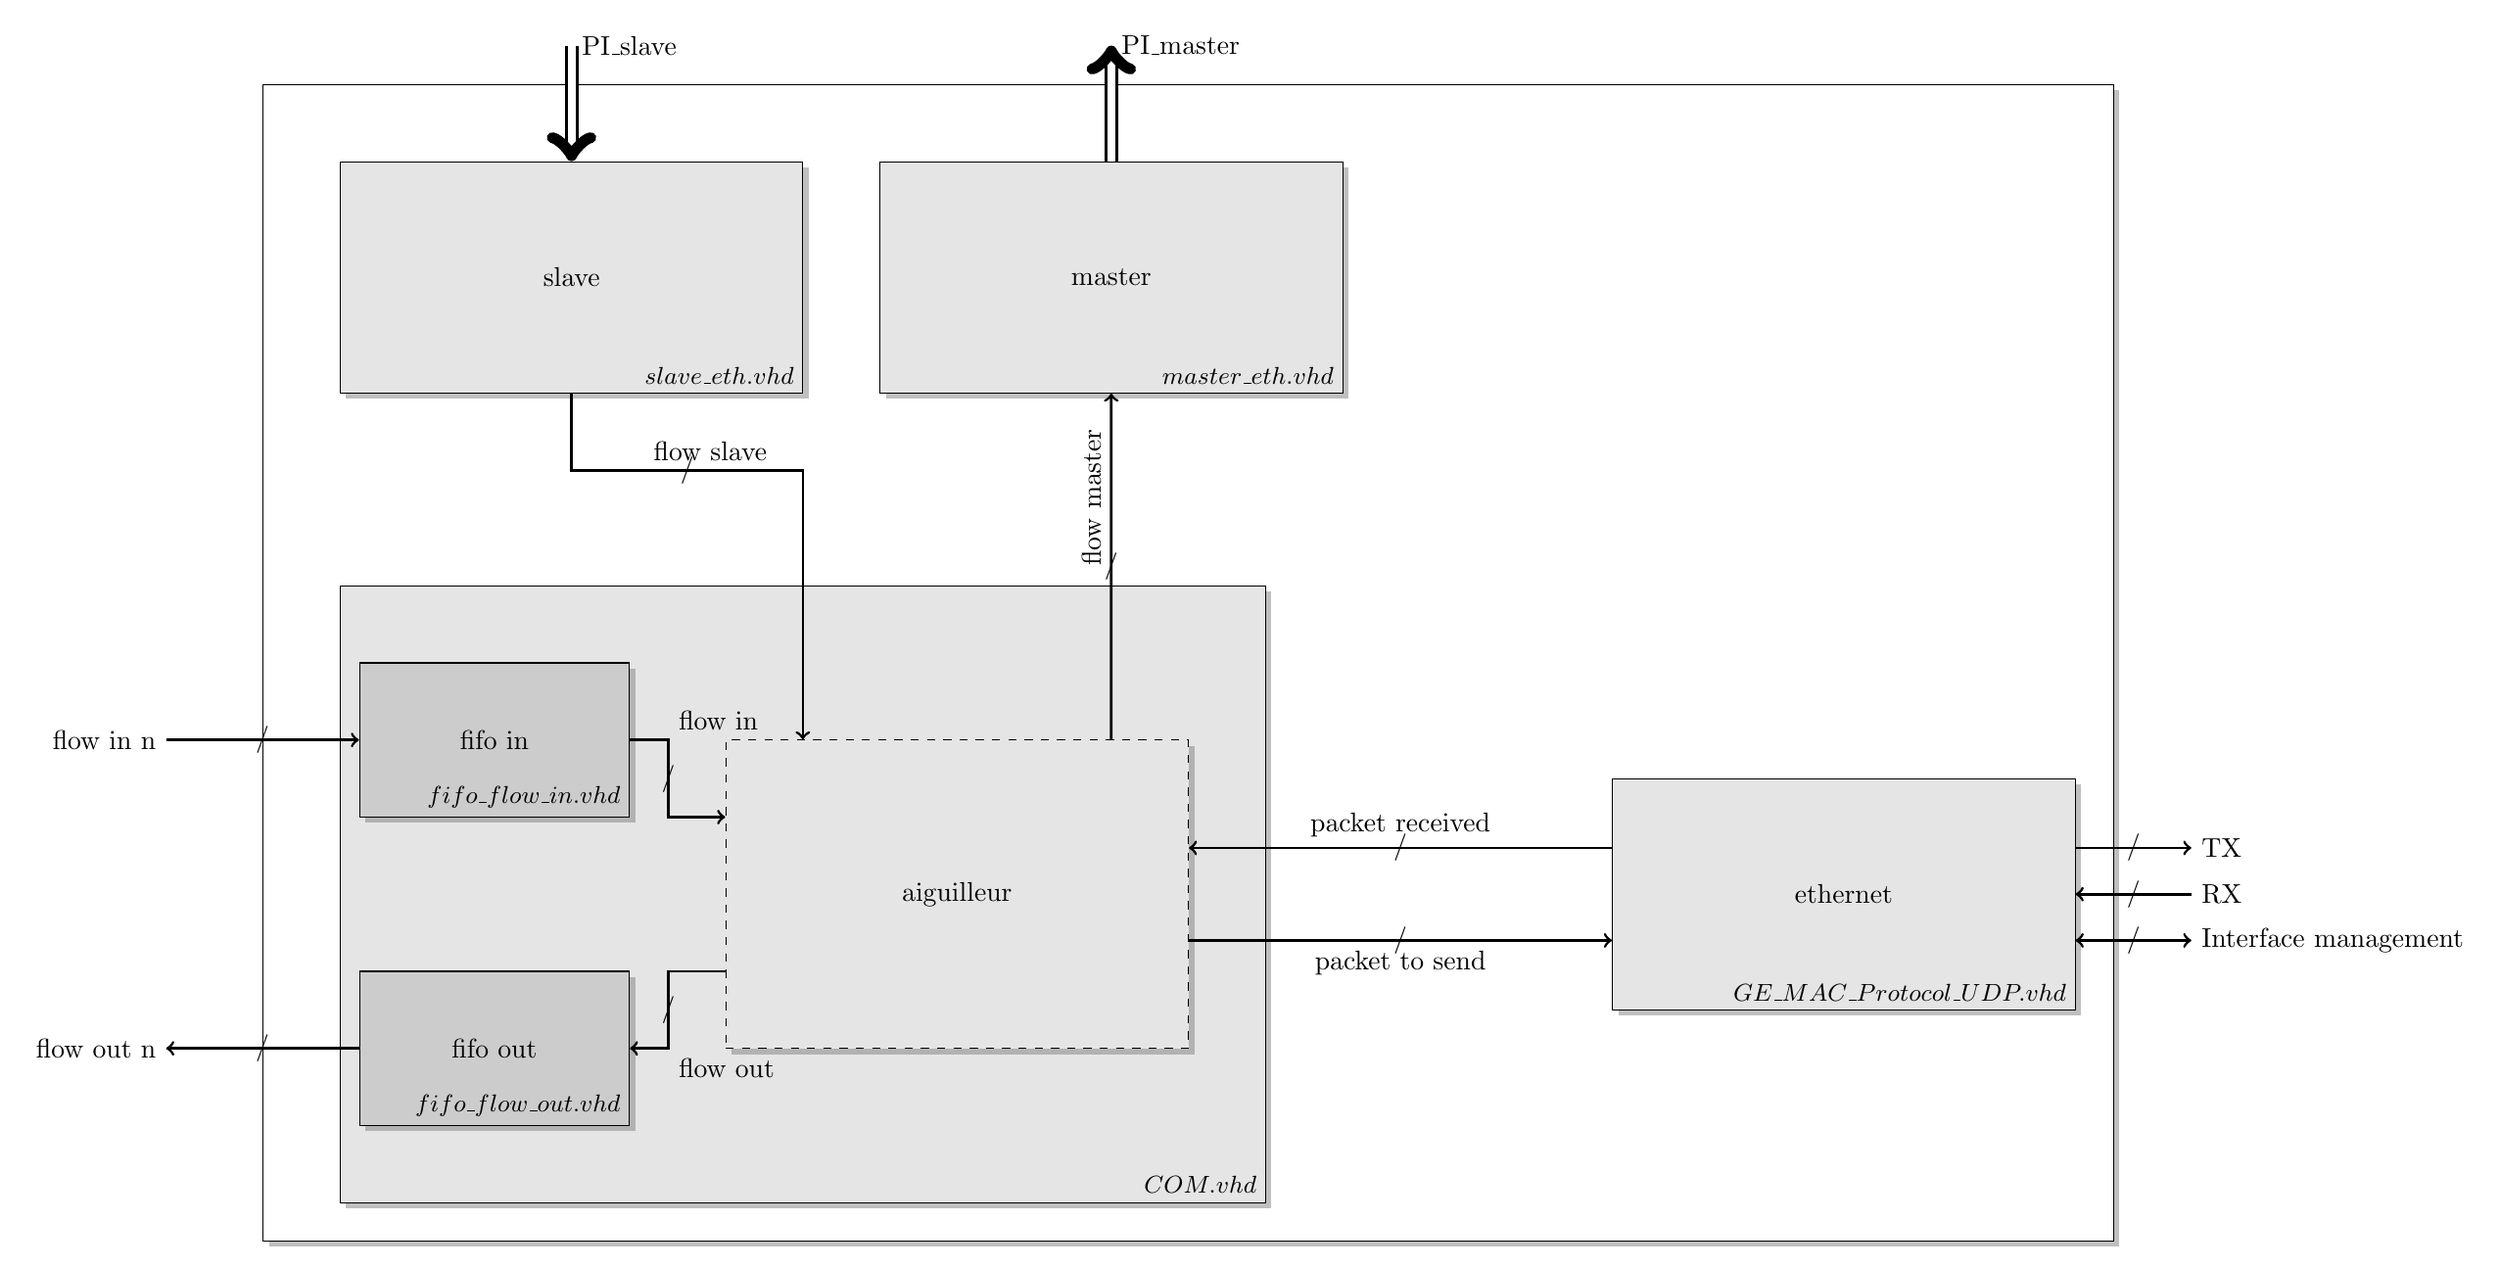
\begin{tikzpicture}



\node[block,minimum height=15cm,minimum width=24cm, fill=white] (bloc) { };

%COM
\node[block,minimum height=8cm,minimum width=12cm, fill=gray!20] (topcom) at([xshift=-5cm,yshift=-3cm]bloc) { };
\draw (topcom.south east) node[above left]{\small $COM.vhd$} ;
%flow in
\node[block,minimum height=2cm,minimum width=3.5cm, fill=gray!40] (fifoin) at([xshift=-4cm,yshift=2cm]topcom) {fifo in };
\draw (fifoin.south east) node[above left]{\small $fifo\_flow\_in.vhd$} ;
\path[connect,<-] (fifoin.west) --  node{/}  ++ (-2.5cm,0) node[left]{flow in n};
%flow out
\node[block,minimum height=2cm,minimum width=3.5cm, fill=gray!40] (fifoout) at([xshift=-4cm,yshift=-2cm]topcom) {fifo out };
\draw (fifoout.south east) node[above left]{\small $fifo\_flow\_out.vhd$} ;
\path[connect,->] (fifoout.west) --  node{/}  ++ (-2.5cm,0) node[left]{flow out n};

%aiguilleur
\node[block,minimum height=4cm,minimum width=6cm,dashed, fill=gray!20] (com) at([xshift=2cm]topcom) {aiguilleur};


%slave master
\node[block,minimum height=3cm,minimum width=6cm, fill=gray!20] (slave) at([xshift=-8cm,yshift=5cm]bloc) {slave};
\draw (slave.south east) node[above left]{\small $slave\_eth.vhd$} ;
\node[block,minimum height=3cm,minimum width=6cm, fill=gray!20] (master) at([xshift=-1cm,yshift=5cm]bloc) {master};
\draw (master.south east) node[above left]{\small $master\_eth.vhd$} ;
\path[connect,<-][double distance = 3pt] (slave.north) --   ++ (0,1.5cm) node[right]{PI\_slave};
\path[connect,->][double distance = 3pt] (master.north) --  ++ (0,1.5cm) node[right]{PI\_master};
\path[connect,<-] (master.south) --  node{/} node[above, pos=0.3,rotate=90]{flow master} ([xshift=2cm]com.north);
\path[connect,->] (slave.south) -| ([yshift=-1cm]slave.south) -|  node[pos=0.25]{/}  node[above, pos=0.3]{flow slave} ([xshift=-2cm]com.north);
%ethernet bloc
\node[block,minimum height=3cm,minimum width=6cm, fill=gray!20] (eth) at([xshift=8.5cm,yshift=-3cm]bloc) {ethernet};
\draw (eth.south east) node[above left]{\small $GE\_MAC\_Protocol\_UDP.vhd$} ;
\path[connect,->] ([yshift=0.6cm]eth.east) --  node{/}  ++ (1.5cm,0) node[right]{TX};
\path[connect,<-] (eth.east) --  node{/}  ++ (1.5cm,0) node[right]{RX};
\path[connect,<->] ([yshift=-0.6cm]eth.east) --  node{/}  ++ (1.5cm,0) node[right]{Interface management};

%internal signals
\path[connect,->] ([yshift=0.6cm]eth.west) --  node{/}  node[above]{packet received} ([yshift=0.6cm]com.east);
\path[connect,<-] ([yshift=-0.6cm]eth.west) --  node{/} node[below]{packet to send} ([yshift=-0.6cm]com.east) ;
\path[connect,->] (fifoin.east) -| ([xshift=0.5cm]fifoin.east) node[above right]{flow in} |-  node[pos=0.25]{/} ([yshift=1cm]com.west) ;
\path[connect,<-] (fifoout.east) -|  ([xshift=0.5cm]fifoout.east) node[below right]{flow out} |- node[pos=0.25]{/} ([yshift=-1cm]com.west) ;



\end{tikzpicture}


\end{document}